\section{Collecte automatisée}
\begin{tcolorbox}[title=Les déchets des uns...]
On dit que les rues du Web sont pavées de données qui n'attendent que la collecte... mais la quantité de déchets qu'on y retrouve est surprenante. \\[-0.6cm]
\begin{flushright}
-- Patrick Boily, 2020
\end{flushright}
\end{tcolorbox}
\noindent Les façons dont les données sont \textbf{partagées}, \textbf{recueillies} et \textbf{publiées} ont bien changé au cours des dernières années en raison de l'omniprésence du \textit{World Wide Web}. Les \textbf{entreprises privées}, les \textbf{gouvernements} et les \textbf{utilisateurs individuels} publient et partagent toutes sortes de données et d'informations. À chaque instant, des mécanismes engendrent de grandes quantités de données.
%Il fut un temps, dans un passé récent, où la rareté et l'inaccessibilité des données constituaient un problème pour les chercheurs et les décideurs. Ce n'est \textbf{définitivement} plus le cas.  
\newl L'abondance des données pose toutefois certains problèmes, notamment en ce qui concerne 
\begin{itemize}[noitemsep]
\item des masses de données enchevêtrées, et 
\item des méthodes traditionnelles de collecte et d'analyse de données qui ne sont plus à la hauteur en raison de leur manque d'efficacité.
\end{itemize}
La popularité et la puissance croissantes des \textbf{logiciels libres}, tels que \text{R} et \text{Python} (dont le code source peut être inspecté, modifié, et amélioré par quiconque), rendent la collecte automatisée de données très attrayante. 

Mais attention: les modules et les librairies de code deviennent \textbf{désuets} en un clin d'œil. Si l'analyste est incapable (ou refuse) de \textbf{maintenir leur programme d'extraction et d'analyse} et de \textbf{surveiller les sites} desquels les données sont extraites, le choix du logiciel ne fera pas, en fin de compte, une grande différence. 
\newpage\noindent
Alors pourquoi prendre la peine d'automatiser la collecte des données? Voici quelques considérations courantes:
\begin{itemize}[noitemsep]
    \item la faiblesse des ressources financières;
    \item le manque de temps ou le désir de recueillir les données manuellement;
\item orte le désir de travailler avec des sources de données actualisées de haute qualité, et  
\item la nécessité de documenter le processus analytique du début (collection) jusqu'à la fin (publication).
\end{itemize} 
La collecte manuelle, en revanche, tend à être encombrante et sujette aux erreurs; les approchess non reproductibles sont également sujettes à des risques accrus de ``mort par ennui'', alors que les solutions programmattiques sont généralement plus fiables, reproductibles, rapides, et produisent des données de meilleure qualité (en supposant que des données cohérente existent au départ). 
\subsection{Liste de contrôle pour la collecte automatisée} Cela dit, le \textbf{raclage de la toile} (web scraping) n'est pas toujours recommandé. En premier lieu, il est possible qu'aucune source de données en ligne et librement accessible ne réponde aux besoins de l'analyse, auquel cas on devrait privilégier une approche d'échantillonnage. \par Cependant, si la réponse à la plupart des questions suivantes est positive, une approche automatisée peut s’avérer être un choix judicieux.
\begin{itemize}[noitemsep]
\item Est-il nécessaire de répéter la tâche de façon périodique (par exemple pour mettre à jour une base de données)?
\item Est-il nécessaire que d'autres analystes soient en mesure de reproduire le processus de collecte?
\item Des sources de données en ligne sont-elles fréquemment utilisées?
\item La tâche est-elle non triviale en termes de portée et de complexité?
\item Si la tâche peut être effectuée manuellement, les ressources financières nécessaires manquent-elles?
\end{itemize}
L'objectif en est simple: la collecte automatique de données devrait permettre d'obtenir des données non structurées (ou non triées), à un prix raisonnable.
\subsection{Consid\'erations d'ordre éthique} Nous nous penchons à présent sur une question brûlante: les données disponibles en ligne sont-elles vraiment libres? 
\par Un \textbf{spider} est un programme qui parcourt rapidement le web à la recherche de données. Il s'aute d'une page à l'autre, en s'emparant de tout leur contenu. Le \textbf{raclage} (scraping), quant a lui, consiste à recueillir des renseignements spécifiques sur des sites  spécifiques: en quoi ces deux concepts sont-ils différents? 
\begin{quote}``Le raclage implique intrinsèquement la \textbf{copie} d’information; l'une des revendications les plus évidentes contre les grattoirs est donc  la violation des droits d'auteur.'' \cite{DC_MRMN}\end{quote}
Que peut-on faire pour minimiser le risque? 
\begin{itemize}[noitemsep]
\item travailler de manière aussi transparente que possible;
\item documenter les sources de données à tout moment;
\item remettre le mérite à ceux qui ont collecté et publié les données au départ;
\item demander l'autorisation de reproduire les informations (si vous ne les avez pas recueillies) et, surtout
\item ne commettre aucun acte illégal.
\end{itemize}
Les tribunaux n'ont pas encore trouvé leur rythme dans ce dossier (consulter, par exemple, \textit{eBay} vs \textit{Bidder's Edge}, \textit{Associated Press} vs \textit{Meltwater}, \textit{Facebook} vs \textit{Pete Warden}, etc. \cite{DC_M}). Il y a plusieurs questions juridiques \`a eétudier, mais il semble en général que les grandes entreprises/organisations sortent généralement victorieuses de ces batailles légales. \par La question est floue par ce qu’il n’est pas évident de différentier les actions de grattage illégales de celles qui sont légales. Il y a des lignes directrices approximatives: la republication de contenu à des fins commerciales est considérée comme plus problématique que le téléchargement de pages pour la recherche et l'analyse, par exemple. Le fichier \texttt{robots.txt} (``Robots Exclusion Protocol'', cf.\@ Figure~\ref{fig:robots}) indique aux gratteurs quelles informations peuvent être recueillies sur le site avec le consentement de leur auteur -- au minimum, il faut en tenir compte, quoique cela n'offre pas une protection absolue.
\begin{figure}[t]
\centering
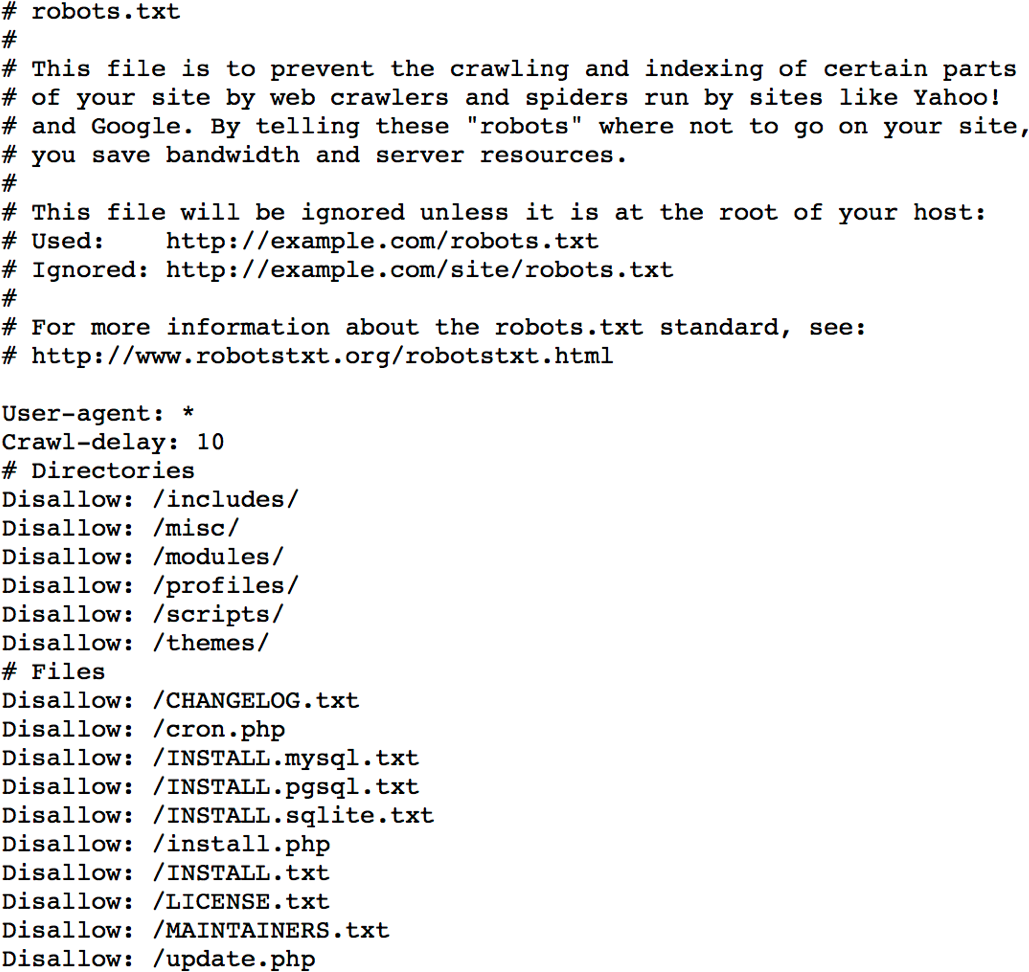
\includegraphics[width=0.50\textwidth]{Images//CQADS_robots.png}
\caption{Fichier \texttt{robots.txt} du site  \newhref{cqads.carleton.ca}{cqads.carleton.ca}.}\hrule\label{fig:robots}
\end{figure}
\afterpage{\FloatBarrier}
\newl Un bon programme de grattage doit 1) se comporter ``convenablement'', 2) fournir des données utiles, et 3) être efficace, dans cet ordre. En cas de doute, contactez les propriétaires du site afin de vérifier s'ils accordent l'accès aux bases de données ou aux fichiers. 
\newpage\noindent Notons finalement l'importance de suivre les \textbf{règles de bienséance} du grattage:
\begin{enumerate}[noitemsep]
    \item \textbf{demeurer identifiable};
    \item \textbf{réduire le trafic} -- accepter les fichiers comprimés, vérifier qu'un fichier a été modifié avant d'y accéder à nouveau, ne récupérer que les parties essentielles;
    \item \textbf{ne pas déranger le serveur avec des requêtes multiples} -- de nombreuses requêtes par seconde peuvent entraîner des pannes de serveur, ce qui peut mener les webmestres à vous bloquer si votre gratteur est trop gourmand (quelques requêtes par seconde suffisent);
    \item \textbf{écrire des grattoirs efficaces et polis} -- il n'y a aucune raison de gratter les pages quotidiennement ou de répéter la même tâche sans cesse… il est préférable de sélectionner des ressources spécifiques et de laisser le reste intact. 
\end{enumerate}
\subsection{Qualité des données de la toile} Le question de la qualité des données est incontournable. Il n'est pas rare de voir des organisations dépenser des milliers de dollars en collecte de données (automatique ou manuelle) mal concue pour ensuite insister que leurs analystes se servent de données défectueuses puisque ce sont les seules données disponibles. \par Ce problème peut être escamoté dans une certaine mesure lorsque les analystes participent aussi à la collecte des données:
\begin{itemize}[noitemsep]
    \item Quel type de données est le mieux adapté pour répondre à aux question de l'organisation?
    \item Les données disponibles sont-elles de qualité suffisante pour donner des reponses utiles aux questions du client?
    \item les informations disponibles sont-elles systématiquement erronées?
\end{itemize}
Sur la toile, les données peuvent provenir de \textbf{sources directes} (un tweet ou un article d'actualité), ou de \textbf{sources indirectes} (copiées d'une source hors ligne ou grattées à partir d’un autre site, ce qui peut rendre leur retraçage difficile). Le \textbf{recoupement de données} (``cross-referencing’’) est une pratique courante lorsqu’on compose avec des données secondaires.  \par La qualité des données dépend également de leur \textbf{usage} et des \textbf{objectifs} d'analyse. Par exemple, 
un échantillon de tweets recueilli un jour quelconque peut être utilisé afin d'analyser l'utilisation de ``hashtags'' spécifiques, mais cet ensemble de données peut s’avérer pratiquement inutile si l’échantillon est recueilli jour d'élection fédérale (en raison du \textbf{bias de collecte}).
\newl Un exemple peut aider à décortiquer les pièges et les défis. Supposons qu'un client souhaite savoir, grâce à une enquête téléphonique typique, ce que les gens pensent d'une nouvelle éplucheuse de patate.  Une telle approche comporte un certain nombre de risques:
\begin{itemize}[noitemsep]
\item\textbf{échantillon non représentatif} -- l'échantillon sélectionné peut ne pas représenter la population visée;
\item\textbf{non-réponse systématique} -- les gens qui n'aiment pas les enquêtes télépho\-ni\-ques peuvent être moins (ou plus) susceptibles d'aimer la nouvelle  éplucheuse;  
\item\textbf{erreur de couverture} -- les gens sans ligne télépho\-ni\-que fixe ne sont pas rejoignables, et \item\textbf{erreur de mesure} -- les questions de l'enquête peuvent ne pas fournir l'information requise.
\end{itemize}
Les solutions classiques à ces problèmes nécessitent le recours à l'échantillonnage, au design de questionnaires, %aux enquêtes omnibus, à des systèmes de récompense, 
etc. Ces solutions peuvent s’avérer  \textbf{coûteuses} et \textbf{inefficaces}. L’utilisation de ``\textbf{proxies}'’ peut aussi être utile -- il s’agit d'indicateurs fortement liés à la popularité d'un produit, telles les statistiques de vente sur un site web commercial. 
\par Le classement des éplucheuse sur \texttt{Amazon.ca} (ou un site web similaire) peut, en fait, dresser un portrait bien plus complet du marché des éplucheuses que ne pourrait le ferait une enquête traditionnelle (en supposant, bien sûr, que l’on fait confiiance à ce dernier). L’information recherchée pourrait donc être obtenue en élaborant un scraper compatible avec l'\textbf{interface de programmation} (API) d'Amazon afin de  recueillir les données appropriées.\newl Il va de soit que cette approche peut également poser certains problèmes: 
\begin{itemize}[noitemsep]
\item \textbf{représentativité} des \textbf{produits listés} -- est-ce que les éplucheuses sont toutes répertoriées? Si ce n'est pas le cas, est-ce parce que ce site web ne les vend pas? Y a-t-il une autre raison?
\item \textbf{représentativité} des \textbf{clients} -- y a-t-il des groupes spécifiques qui achètent (ou non) de produits en ligne? Y a-t-il des groupes spécifiques qui achètent sur des sites spécifiques? Y a-t-il des groupes spécifiques qui laissent (ou non) des critiques de produits? 
\item \textbf{fiabilité} des clients et des critiques -- comment dis\-tin\-gue-t-on les fausses critques des critiques réelles?
\end{itemize}
Le scraping est généralement bien adapté à la collecte de données sur les produits, mais il existe plusieurs situations pour lesquelles il est nettement plus difficile d'imaginer où trouver des données en ligne: quelles données pourriez-vous collecter en ligne afin de mesurer la popularité d'une politique gouvernementale, par exemple? 
\subsection{Technologies du web: premiers pas}
En lignes, les données se trouvent sous forme de \textbf{textes}, de \textbf{tableaux}, de \textbf{listes}, de \textbf{liens} et autres structures, mais elles ne sont pas présentées dans les fureteurs de la même manière qu'elles sont stockées en HTML/XML. De plus, lorsque les pages web sont \textbf{dynamiques}, il y a un "coût" associé à la collecte automatisée. Par conséquent, une connaissance de base du web et de ses technologies est cruciale. Des renseignements sont facilement accessibles en ligne (cf.\@ références) et dans \cite{DC_M,DC_MRMN}.\newpage\noindent There are three areas of importance for data collection on the web:
\begin{itemize}[noitemsep]
\item technologies for \textbf{content dissemination} (HTTP, HTML/XML, JSON, plain text, etc.);
\item technologies for \textbf{information extraction} (R, Python XPath, JSon parsers, Beautiful Soup, Selenium, regexps, etc.), and 
\item technologies for \textbf{data storage} (R, Python, SQL, binary formats, plain text formats, etc.).
\end{itemize}
Webpage content itself comes into three main categories: Hypertext Markup Language (HTML; used for web content and code), Cascading Style Sheets (CSS; used for webpage style), and 
JavaScript (js; used for interactivity with the webpage). HTML is, in some sense, the most fundamental; understanding the tree structure of HTML documents, for instance, will go a long way towards helping consultants get full use of the \textbf{scraping toolbox}. 
\subsection{Scraping Toolbox} Our experience has shown that a number of tools can facilitate the automated data extraction process, including: 
\textit{Developer Tools}, \textit{XPath}, \textit{Beautiful Soup}, \textit{Selenium}, and \textit{regular expressions}. 
\newl\textbf{Developer Tools} show the correspondence between the HTML code for a page and the rendered version seen in the browser (see Figure~\ref{fig:erb} for an example). Unlike ``View Source'', Developer Tools show the \textit{dynamic} version of the HTML content (i.e. the HTML is shown with any changes made by JavaScript since the page was first received). Inspecting a page's various elements and discovering where they reside in the HTML file is \textbf{crucial} to efficient web scraping: 
\begin{figure*}[t]
\centering
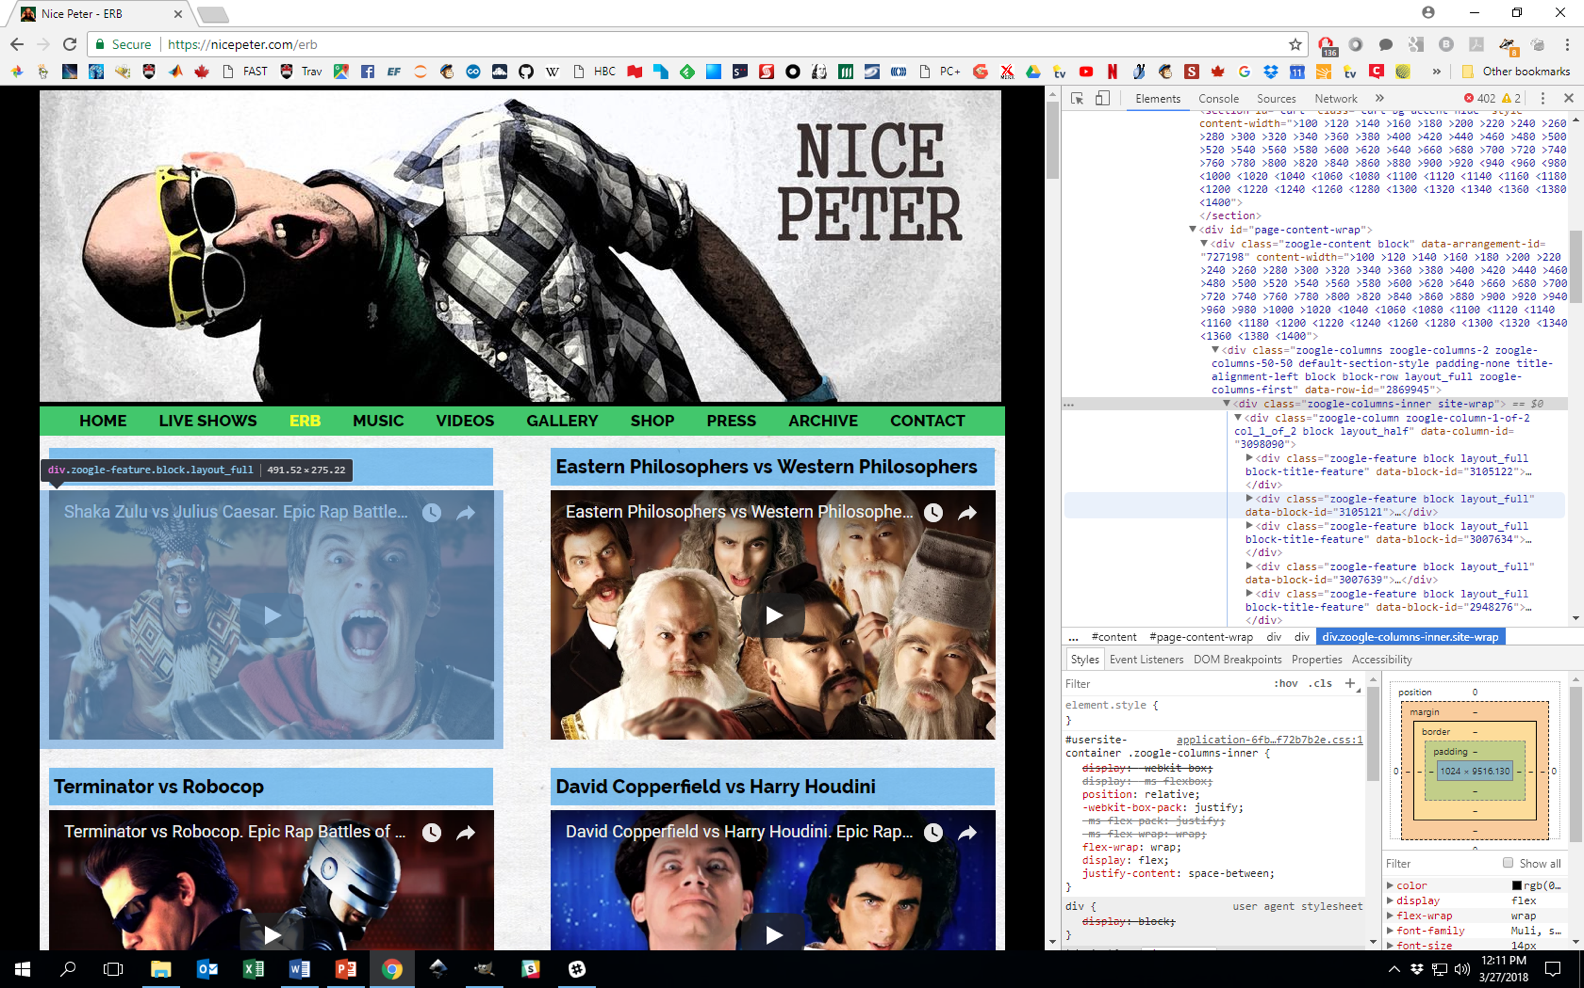
\includegraphics[width=\textwidth]{Images//erb.png}
\caption[\small Inspecting a webpage elements using Chrome's \textit{Developer Tools}]{\small Inspecting \newhref{https://nicepeter.com/erb}{https://nicepeter.com/erb}'s elements using Chrome's \textit{Developer Tools}.} \hrule\label{fig:erb}
\end{figure*}
\begin{itemize}[noitemsep]
\item \textbf{Firefox} -- right click page $\to$ Inspect Element
\item \textbf{Safari} -- Safari $\to$ Preferences $to$ Advanced $\to$ Show Develop Menu in Menu Bar, then  
Develop $\to$ Show Web Inspector
\item \textbf{Chrome} --  right click page $\to$ Inspect
\end{itemize}
\textbf{XPath} is a query (domain-specific) language which is 
used to select specific pieces of information from marked-up documents such as HTML, XML, or variants such as SVG, RSS. Before this can be done, the information stored in a marked-up document needs to be converted (or \textbf{parsed}) into a format suitable for processing and statistical analysis; this is implemented in the R package XML, for instance. The process is simple; it involves 
\begin{enumerate}[noitemsep]
\item specifying the data of interest;
\item locating it in a specific document, and
\item tailoring a query to the document to extract the desired info.
\end{enumerate}
XPath queries require both a \textbf{path} and a \textbf{document} to search; paths consist of hierarchical addressing mechanism (succession of nodes, separated by forward slashes (``/''), while a query takes the form \small\texttt{xpathSApply(doc,path)}\normalsize :\\
\footnotesize\texttt{xpathSApply(parsed\_doc,``/html/body/div/p/i'')}\normalsize, for instance, would find all \texttt{<i>} tags found inside a \texttt{<p>} tag, itself found inside a \texttt{<div>} tag in the \texttt{body} of the \texttt{html} file of \texttt{parsed\_doc}. Consult \cite{DC_MRMN} for a substantially heftier introduction. 
\newl\textbf{Regular Expressions} can be used to achieve the main web scraping objective, which is to extract  relevant information from reams of data. Among this mostly unstructured data lurk \textbf{systematic elements}, which can be used to help the automation process, especially if quantitative methods are eventually going to be applied to the scraped data. Systematic structures include numbers, names (countries, etc.), addresses (mailing, e-mailing, URLs, etc.), specific character strings, etc. Regular expressions (regexps) are abstract sequences of strings that match concrete recurring patterns in text; they allow for the systematic extraction of the information components from plain text, HTML, and XML. Some examples that illustrate the main concepts are shown in the accompanying \textit{Jupyter Notebooks} %showcased in Section~\ref{sec:docs}. 
\newl\textbf{Beautiful Soup} is a Python library that helps extract data out of HTML and XML files. It parses HTML files, even if they're broken. Beautiful Soup does not simply convert bad HTML to good X/HTML; it allows a user to fully inspect the (proper) HTML structure it produces, in a programmatical fashion. When Beautiful Soup has finished its work on an HTML file, the resulting \textit{soup} is an API for \textbf{traversing}, \textbf{searching}, and \textbf{reading} the document's elements. In essence, it provides \textbf{idiomatic} ways of navigating, searching, and modifying the parse tree of the HTML file, which can save a fair amount of time.
\par For instance, \texttt{soup.find\_all('a')} would find and output all \texttt{<a ...> ... </a>} tag pairs (with attributes and content) in the \texttt{soup}, whereas \begin{quote}\texttt{for link in soup.find\_all('a'):}\newline \texttt{\ \ \ print(link.get('href')}
\end{quote} would output the URLs found in the same tag pairs. The Beautiful Soup documentation is quite explicit and provides numerous examples \cite{DC_BS}. 
\newl\textbf{Selenium} is a Python tool used to automate web browser interactions.  It is used primarily for testing purposes, but it has data extraction uses as well. Mainly, it allows the user to open a browser and to act as a human being would:
\begin{itemize}[noitemsep]
    \item clicking buttons;
\item entering information in forms;
\item searching for specific information on a page, etc.
\end{itemize}
Selenium requires a driver to interface with the chosen browser. Firefox, for example, uses \texttt{geckodriver}. Other supported browsers have their own drivers (see \cite{DC_S_C,DC_S_E,DC_S_F,DC_S_S}).

\noindent Selenium automatically controls a complete browser, including rendering the web documents and running JavaScript. This is useful for pages with a lot of dynamic content that isn't in the base HTML. Selenium can program actions like ``click on this button'', or ``type this text'', to provide access to the dynamic HTML of the current state of the page, not unlike what happens in  \textit{Developer Tools} (but now the process can be fully automated). More information can be found in \cite{DC_S,DC_S2}.
\newl 
Let us end this section by providing a short summary of the \textbf{automated data collection decision process} \cite{DC_MRMN,DC_M}, as seen by  quantitative consultants. 
\begin{enumerate}
    \item \textbf{Know exactly what kind of information the client needs}, either \textbf{specific} (e.g. GDP of all OECD countries for last 10 years, sales of top 10 tea brands in 2017, etc.) or \textbf{vague} (people's opinion on tea brand $X$, etc.)
\item \textbf{Find out if there are any web data sources that could provide direct or indirect information on the client's problem.} That is easier to achieve for specific facts (a tea store's webpage will provide information about teas that are currently in demand) than it is for vague facts. Tweets and social media platforms may contain opinion trends; commercial platforms can provide information on product satisfaction.
\item \textbf{Develop a theory of the data generation process when looking into potential data sources.} When was the data generated? When was it uploaded to the Web? Who uploaded the data? Are there any potential areas that are not covered, consistent, or accurate? How often is the data updated?
\item \textbf{Balance the advantages and disadvantages of potential data sources.} Validate the quality of data used -- are there other independent sources that provide similar information against which to crosscheck? Can original source of secondary data be identified?
\item \textbf{Make a data collection decision}. Choose the data sources that seem most suitable, and document reasons for this decision. Collect data from several sources to validate the final choice. 
\end{enumerate}
%\afterpage{\FloatBarrier}